\documentclass{standalone}
\usepackage{tikz}
\usetikzlibrary{patterns, positioning}
\usetikzlibrary{shapes.misc}
\usepackage[outline]{contour}
\contourlength{1.5pt} 
\usepackage[sfdefault]{ClearSans} %% option 'sfdefault' activates Clear Sans as the default text font
\usepackage[T1]{fontenc}

\begin{document}
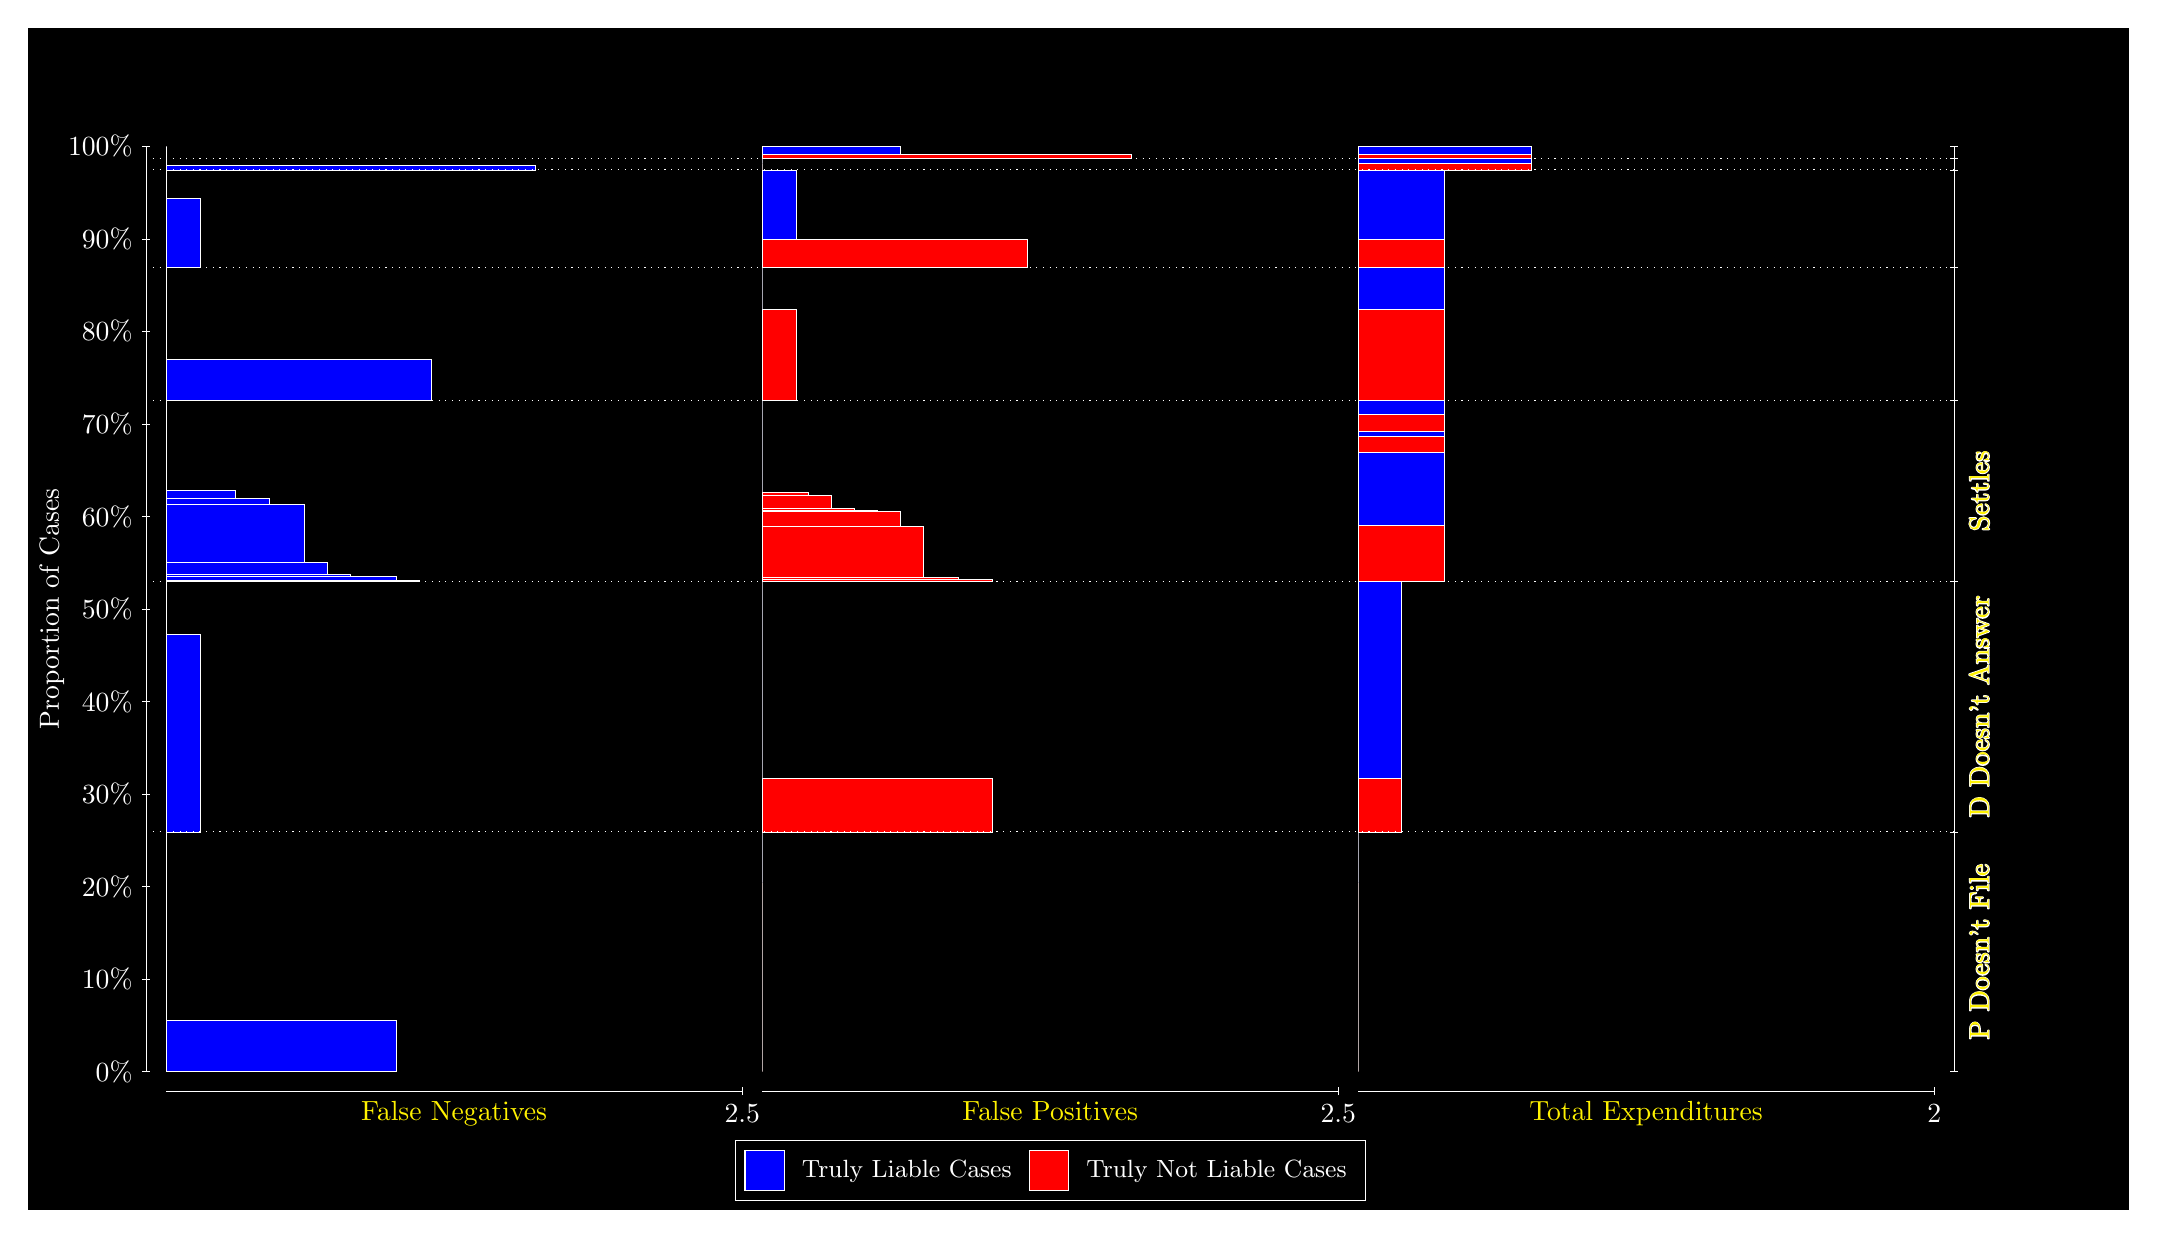
\begin{tikzpicture}
\draw[fill=black] (0,0) rectangle (26.667,15);
\draw[white, very thin] (1.5,1.75) -- (1.5,13.5);
\node[rotate=90, text=white, anchor=center] at (0.3, 7.625) {Proportion of Cases};
\draw[white, very thin] (1.45,1.75) -- (1.55,1.75);
\node[text=white, anchor=east] at (1.45, 1.75) {0\%};
\draw[white, very thin] (1.45,2.925) -- (1.55,2.925);
\node[text=white, anchor=east] at (1.45, 2.925) {10\%};
\draw[white, very thin] (1.45,4.1) -- (1.55,4.1);
\node[text=white, anchor=east] at (1.45, 4.1) {20\%};
\draw[white, very thin] (1.45,5.275) -- (1.55,5.275);
\node[text=white, anchor=east] at (1.45, 5.275) {30\%};
\draw[white, very thin] (1.45,6.45) -- (1.55,6.45);
\node[text=white, anchor=east] at (1.45, 6.45) {40\%};
\draw[white, very thin] (1.45,7.625) -- (1.55,7.625);
\node[text=white, anchor=east] at (1.45, 7.625) {50\%};
\draw[white, very thin] (1.45,8.8) -- (1.55,8.8);
\node[text=white, anchor=east] at (1.45, 8.8) {60\%};
\draw[white, very thin] (1.45,9.975) -- (1.55,9.975);
\node[text=white, anchor=east] at (1.45, 9.975) {70\%};
\draw[white, very thin] (1.45,11.15) -- (1.55,11.15);
\node[text=white, anchor=east] at (1.45, 11.15) {80\%};
\draw[white, very thin] (1.45,12.325) -- (1.55,12.325);
\node[text=white, anchor=east] at (1.45, 12.325) {90\%};
\draw[white, very thin] (1.45,13.5) -- (1.55,13.5);
\node[text=white, anchor=east] at (1.45, 13.5) {100\%};

\draw[white, very thin] (24.457,1.75) -- (24.457,13.5);
\draw[white, very thin] (24.407,1.75) -- (24.507,1.75);
\node[anchor=west] at (24.407, 1.75) {};
\draw[white, very thin] (24.407,4.7944) -- (24.507,4.7944);
\node[anchor=west] at (24.407, 4.7944) {};
\draw[white, very thin] (24.407,7.9766) -- (24.507,7.9766);
\node[anchor=west] at (24.407, 7.9766) {};
\draw[white, very thin] (24.407,10.27) -- (24.507,10.27);
\node[anchor=west] at (24.407, 10.27) {};
\draw[white, very thin] (24.407,11.958) -- (24.507,11.958);
\node[anchor=west] at (24.407, 11.958) {};
\draw[white, very thin] (24.407,13.202) -- (24.507,13.202);
\node[anchor=west] at (24.407, 13.202) {};
\draw[white, very thin] (24.407,13.342) -- (24.507,13.342);
\node[anchor=west] at (24.407, 13.342) {};
\draw[white, very thin] (24.407,13.5) -- (24.507,13.5);
\node[anchor=west] at (24.407, 13.5) {};

\draw[white, very thin, fill=blue] (1.75,1.75) rectangle (4.6775,2.3964);
\draw[white, very thin, fill=red] (1.75,2.3964) rectangle (1.75,4.7944);
\draw[white, very thin, fill=blue] (1.75,4.7944) rectangle (2.1891,7.2986);
\draw[white, very thin, fill=red] (1.75,7.2986) rectangle (1.75,7.9766);
\draw[white, very thin, fill=blue] (1.75,7.9766) rectangle (4.9703,7.9878);
\draw[white, very thin, fill=blue] (1.75,7.9878) rectangle (4.6775,8.0337);
\draw[white, very thin, fill=blue] (1.75,8.0337) rectangle (4.3848,8.0427);
\draw[white, very thin, fill=blue] (1.75,8.0427) rectangle (4.092,8.0588);
\draw[white, very thin, fill=blue] (1.75,8.0588) rectangle (3.7993,8.2212);
\draw[white, very thin, fill=blue] (1.75,8.2212) rectangle (3.5065,8.9582);
\draw[white, very thin, fill=blue] (1.75,8.9582) rectangle (3.0674,9.0246);
\draw[white, very thin, fill=blue] (1.75,9.0246) rectangle (2.6283,9.1339);
\draw[white, very thin, fill=red] (1.75,9.1339) rectangle (1.75,10.27);
\draw[white, very thin, fill=blue] (1.75,10.27) rectangle (5.1167,10.801);
\draw[white, very thin, fill=red] (1.75,10.801) rectangle (1.75,11.958);
\draw[white, very thin, fill=blue] (1.75,11.958) rectangle (2.1891,12.838);
\draw[white, very thin, fill=red] (1.75,12.838) rectangle (1.75,13.202);
\draw[white, very thin, fill=blue] (1.75,13.202) rectangle (6.4341,13.262);
\draw[white, very thin, fill=red] (1.75,13.262) rectangle (1.75,13.342);
\draw[white, very thin, fill=red] (1.75,13.342) rectangle (1.75,13.404);
\draw[white, very thin, fill=blue] (1.75,13.404) rectangle (1.75,13.5);
\draw[white, very thin, fill=red] (9.3189,1.75) rectangle (9.3189,4.148);
\draw[white, very thin, fill=blue] (9.3189,4.148) rectangle (9.3189,4.7944);
\draw[white, very thin, fill=red] (9.3189,4.7944) rectangle (12.246,5.4723);
\draw[white, very thin, fill=blue] (9.3189,5.4723) rectangle (9.3189,7.9766);
\draw[white, very thin, fill=red] (9.3189,7.9766) rectangle (12.246,7.9989);
\draw[white, very thin, fill=red] (9.3189,7.9989) rectangle (11.807,8.0305);
\draw[white, very thin, fill=red] (9.3189,8.0305) rectangle (11.368,8.6691);
\draw[white, very thin, fill=red] (9.3189,8.6691) rectangle (11.075,8.8617);
\draw[white, very thin, fill=red] (9.3189,8.8617) rectangle (10.783,8.8835);
\draw[white, very thin, fill=red] (9.3189,8.8835) rectangle (10.49,8.9014);
\draw[white, very thin, fill=red] (9.3189,8.9014) rectangle (10.197,9.0674);
\draw[white, very thin, fill=red] (9.3189,9.0674) rectangle (9.9044,9.1126);
\draw[white, very thin, fill=blue] (9.3189,9.1126) rectangle (9.3189,10.27);
\draw[white, very thin, fill=red] (9.3189,10.27) rectangle (9.758,11.426);
\draw[white, very thin, fill=blue] (9.3189,11.426) rectangle (9.3189,11.958);
\draw[white, very thin, fill=red] (9.3189,11.958) rectangle (12.686,12.321);
\draw[white, very thin, fill=blue] (9.3189,12.321) rectangle (9.758,13.202);
\draw[white, very thin, fill=red] (9.3189,13.202) rectangle (9.3189,13.283);
\draw[white, very thin, fill=blue] (9.3189,13.283) rectangle (9.3189,13.342);
\draw[white, very thin, fill=red] (9.3189,13.342) rectangle (14.003,13.404);
\draw[white, very thin, fill=blue] (9.3189,13.404) rectangle (11.075,13.5);
\draw[white, very thin, fill=red] (16.888,1.75) rectangle (16.888,4.148);
\draw[white, very thin, fill=blue] (16.888,4.148) rectangle (16.888,4.7944);
\draw[white, very thin, fill=red] (16.888,4.7944) rectangle (17.437,5.4723);
\draw[white, very thin, fill=blue] (16.888,5.4723) rectangle (17.437,7.9766);
\draw[white, very thin, fill=red] (16.888,7.9766) rectangle (17.986,8.687);
\draw[white, very thin, fill=blue] (16.888,8.687) rectangle (17.986,9.6086);
\draw[white, very thin, fill=red] (16.888,9.6086) rectangle (17.986,9.8198);
\draw[white, very thin, fill=blue] (16.888,9.8198) rectangle (17.986,9.8769);
\draw[white, very thin, fill=red] (16.888,9.8769) rectangle (17.986,10.091);
\draw[white, very thin, fill=blue] (16.888,10.091) rectangle (17.986,10.27);
\draw[white, very thin, fill=red] (16.888,10.27) rectangle (17.986,11.426);
\draw[white, very thin, fill=blue] (16.888,11.426) rectangle (17.986,11.958);
\draw[white, very thin, fill=red] (16.888,11.958) rectangle (17.986,12.321);
\draw[white, very thin, fill=blue] (16.888,12.321) rectangle (17.986,13.202);
\draw[white, very thin, fill=red] (16.888,13.202) rectangle (19.083,13.283);
\draw[white, very thin, fill=blue] (16.888,13.283) rectangle (19.083,13.342);
\draw[white, very thin, fill=red] (16.888,13.342) rectangle (19.083,13.404);
\draw[white, very thin, fill=blue] (16.888,13.404) rectangle (19.083,13.5);
\draw[white, dotted] (1.5,4.7944) -- (24.457,4.7944);
\draw[white, dotted] (1.5,7.9766) -- (24.457,7.9766);
\draw[white, dotted] (1.5,10.27) -- (24.457,10.27);
\draw[white, dotted] (1.5,11.958) -- (24.457,11.958);
\draw[white, dotted] (1.5,13.202) -- (24.457,13.202);
\draw[white, dotted] (1.5,13.342) -- (24.457,13.342);
\draw[white, very thin] (1.75,1.5) -- (9.0689,1.5);
\node[text=yellow, anchor=north] at (5.4094, 1.5) {False Negatives};
\draw[white, very thin] (9.0689,1.45) -- (9.0689,1.55);
\node[text=white, anchor=north] at (9.0689, 1.45) {2.5};

\draw[white, very thin] (9.3189,1.5) -- (16.638,1.5);
\node[text=yellow, anchor=north] at (12.978, 1.5) {False Positives};
\draw[white, very thin] (16.638,1.45) -- (16.638,1.55);
\node[text=white, anchor=north] at (16.638, 1.45) {2.5};

\draw[white, very thin] (16.888,1.5) -- (24.207,1.5);
\node[text=yellow, anchor=north] at (20.547, 1.5) {Total Expenditures};
\draw[white, very thin] (24.207,1.45) -- (24.207,1.55);
\node[text=white, anchor=north] at (24.207, 1.45) {2};

\node[text=yellow, centered, rotate=90] at (24.777, 3.2722) {\contour{white}{P Doesn't File}};
\node[text=yellow, centered, rotate=90] at (24.777, 6.3855) {\contour{white}{D Doesn't Answer}};
\node[text=yellow, centered, rotate=90] at (24.777, 9.1232) {\contour{white}{Settles}};





\draw (12.978300999999998,1.5) node[draw=none] (baseCoordinate) {};
\begin{scope}[align=center]
        \matrix[scale=0.5, draw=white, below=0.5cm of baseCoordinate, nodes={draw}, column sep=0.1cm]{
            \node[rectangle, draw, minimum width=0.5cm, minimum height=0.5cm, fill=blue] {}; &
            \node[draw=none, font=\small, text=white] (B) {Truly Liable Cases}; &
            \node[rectangle, draw, minimum width=0.5cm, minimum height=0.5cm, fill=red] {}; &
            \node[draw=none, font=\small, text=white] (B) {Truly Not Liable Cases}; \\
            };
\end{scope}

\end{tikzpicture}
\end{document}